%%
% 结论
% 结论是毕业论文的总结,是整篇论文的归宿,应精炼、准确、完整。结论应着重阐述自己的创造性成果及其在本研究领域中的意义、作用,还可进一步提出需要讨论的问题和建议。
% modifyer: 黄俊杰(huangjj27, 349373001dc@gmail.com)
% update date: 2017-04-13
%%

\chapter{总结与展望}
\section{工作总结}
\section{研究展望}
\section{模板提供的命令}
冒号前面是命令,后面是显示的结果\\

pozhehao(破折号):\pozhehao \sysuspace mybold\{com\}(加粗斜体):\mybold{com} \sysuspace  etoday:\etoday\sysuspace ctoday:\ctoday\sysuspace


用于equation环境的命令

$norm :\norm{t}$

$argmax:\argmax{x}{y}\sysuspace argmin:\argmin{x}{y}$

$varmax:\varmax{x}{y}\sysuspace  varmin:\varmin{x}{y}$

$fncmax:\fncmax{x}{y}\sysuspace  fncmin:\fncmin{x}{y}$

$xxFnorm:\xxFnorm{x}\sysuspace xxFnormSqr:\xxFnormSqr{x}\sysuspace xxFprod:\xxFprod{x}{y}$

$xxOpVec:\xxOpVec{x}\sysuspace xxLprod:\xxLprod{x}{y}\sysuspace xxLprodVec:\xxLprodVec{x}{y}\sysuspace xxTensor:\xxTensor{x}$

$xxBracketY:\xxBracketY{x}\sysuspace xxBracketF:\xxBracketF{x}\sysuspace xxBracketH:\xxBracketH{x}$

\begin{figure}
	\centering
	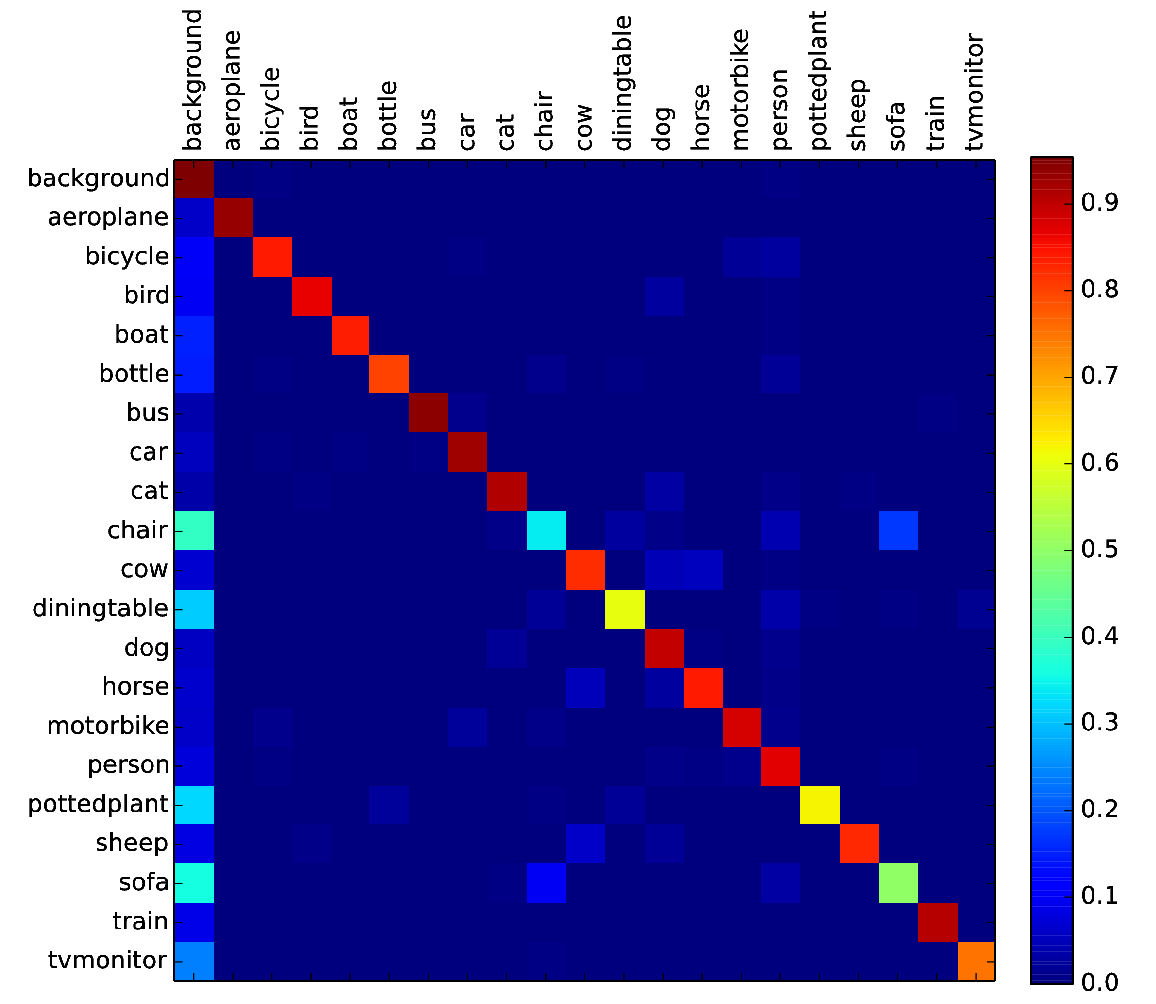
\includegraphics[width=0.5\textwidth]{image/result/confusion.pdf}
	\caption{镶嵌在文中的图像}
	\captionce[图注]{这是测试图注。}{A testing figure legend.}\label{fig:test}
	\label{fig:confusion}
\end{figure}